


%-----------------------------------------------------------
%--- Header
%-----------------------------------------------------------


\documentclass[aspectratio=169, 14pt]{beamer}
\usepackage[utf8]{inputenc}
\usepackage[T1]{fontenc}
\usepackage{eso-pic, picture}
\usepackage{pgf}
\usepackage[absolute, overlay]{textpos}
\usepackage{hyperref}
\usepackage{amsmath}
\usepackage{nccmath}
\usepackage[export]{adjustbox} %%% generating colored frame around image (e.g.: \includegraphics[width=0.45\paperwidth, cfbox=white 3pt 0pt]{/path/to/image.jpg})
\usepackage[official]{eurosym} % use the official € symbol by typing "\euro{}"


% implementing my custom beamer template
\usetheme{daniels}


%-----------------------------------------------------------
%--- Table
%-----------------------------------------------------------


\usepackage{tabularx}
\usepackage{booktabs}
\newcolumntype{L}[1]{>{\raggedright\arraybackslash}p{#1}} % linksb�ndig mit Breitenangabe
\newcolumntype{C}[1]{>{\centering\arraybackslash}p{#1}} % zentriert mit Breitenangabe
\newcolumntype{R}[1]{>{\raggedleft\arraybackslash}p{#1}} % rechtsb�ndig mit Breitenangabe





%-----------------------------------------------------------
%--- Presentation
%-----------------------------------------------------------


\begin{document}


% Title Slide
\title{Einführung in die\\ moderne Digitalelektronik}
\subtitle{Tutorium zur Vorlesung:}
\date{Blockveranstaltung im Sommersemester 2021}
\author{D{\fontsize{10}{10}\selectfont ANIEL} B{\fontsize{10}{10}\selectfont AUR}\\ \texttt{daniel.baur@physik.uni-freiburg.de}}
\begin{frame}
    \titlepage
    %\stepcounter{framenumber}
    \setcounter{framenumber}{0}
\end{frame}


% chapter: MonXe
%\begin{frame}
%    \chapterslide{Radon Emanation Chamber}
%    %\stepcounter{framenumber}
%\end{frame}


% chapter: SFS
%\begin{frame}
%    \chapterslide{Signal Formation Simulations}
%\end{frame}


% Tutorvorstellung: Daniel Baur
\begin{frame}
    \summaryslide{Tutor: Daniel Baur}
    \begin{textblock*}{2\paperwidth}(0.22\paperwidth,0.0\paperheight)
        \vspace*{2.0cm}
        \begin{itemize}
            \setlength\itemsep{16pt}
            \item Arbeitsgruppe: \textcolor{uniblau}{\href{https://www.app.uni-freiburg.de/}{Astroteilchenphysik ({\fontsize{14}{10}\selectfont S}{\fontsize{8}{10}\selectfont CHUMANN} \& {\fontsize{14}{10}\selectfont F}{\fontsize{8}{10}\selectfont ISCHER})}}
            \item E-Mail: \texttt{daniel.baur@physik.uni-freiburg.de}
            \item Hausruf: +49 761 203-5694
            \item Büro: Physik-Hochhaus, Zimmer 607
        \end{itemize}
    \end{textblock*}
    \AddToShipoutPictureBG*{\put(-0.005\paperwidth,0.168\paperheight){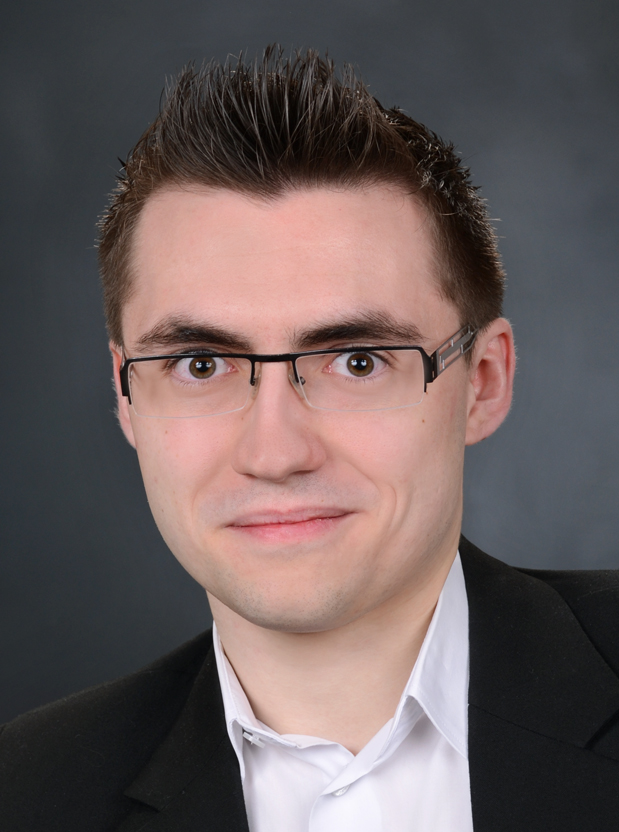
\includegraphics[width=0.25\paperwidth]{./images/Bewerbungsfoto_crop1.jpg}}}
\end{frame}


% Inhaltsverzeichnis
\begin{frame}[label=inhalt]
    \summaryslide{Einführung in die moderne Digitalelektronik: Übungen}
    \begin{textblock*}{2\paperwidth}(0.0\paperwidth,0.0\paperheight)
        \vspace*{1.9cm}
        \begin{itemize}
            \setlength\itemsep{16pt}
            \item \hyperlink{stuff}{Formalia \& Stuff}
            \item \hyperlink{loetuebung}{Lötpraxis}
            \item \hyperlink{boolschealgebra}{Boolsche Algebra}
            \item \hyperlink{fpga}{Einführung in die FPGA-Programmierung}
            \item \hyperlink{mikrocontroller}{Einführung in die Mikrocontroller-Programmierung}
        \end{itemize}
    \end{textblock*}
    %\framenumbersummaryslide
    %\addtocounter{framenumber}{-1}
    \setcounter{framenumber}{0}
\end{frame}


%chapter: Stuff
\begin{frame}[label=stuff]
    \chapterslide{\hyperlink{inhalt}{Formalia \& Stuff}}
    \addtocounter{framenumber}{-1}
\end{frame}


% Formalia
\begin{frame}
    \frametitle{Formalia}
    \begin{textblock*}{2\paperwidth}(0.0\paperwidth,0.0\paperheight)
        \vspace*{2.0cm}
        \begin{itemize}
            \setlength\itemsep{16pt}
            \item Leistung:
            \begin{itemize}
                \item 5 ECTS (Studienleistung): Teilnahme +Kurzvortrag
                \item 7 ECTS (Prüfungsleistung): Teilnahme +Kurzvortrag +Prüfung
            \end{itemize}
            \item Covid-19 $\quad\Rightarrow\quad$ Sitzplätze beibehalten +MNS
            \item Unterlagen: \textcolor{uniblau}{\href{https://ilias.uni-freiburg.de/ilias.php?ref_id=1481157&cmdClass=ilrepositorygui&cmdNode=yh&baseClass=ilrepositorygui}{ILIAS-Kursseite}}
        \end{itemize}
    \end{textblock*}
    \framenumber
\end{frame}


% Literaturempfehlungen
\begin{frame}
    \frametitle{Literaturempfehlungen}
    \begin{textblock*}{2\paperwidth}(0.0\paperwidth,0.0\paperheight)
        \vspace*{2.0cm}
        \begin{itemize}
            \setlength\itemsep{16pt}
            \item Grundlagen: \textcolor{uniblau}{\href{https://link.springer.com/book/10.1007/978-3-662-49731-9}{K{\fontsize{10}{10}\selectfont LAUS} U{\fontsize{10}{10}\selectfont RBANSKI} et al.: Digitaltechnik (7. Auflage)}}
            \item Ergänzung: \textcolor{uniblau}{\href{https://www.youtube.com/playlist?list=PLH2l6uzC4UEW0s7-KewFLBC1D0l6XRfye}{Crash Course: Computer Science}}
            %\item Inspiration: \textcolor{uniblau}{\href{https://www.arduino.cc/}{Arduino Webpage}}
        \end{itemize}
    \end{textblock*}
    \framenumber
\end{frame}


% Zeitplan
\begin{frame}
    \frametitle{Zeitplan der Übungen}
    \begin{textblock*}{\paperwidth}(0.0\paperwidth,0.185\paperheight)
        {\fontsize{12}{10}\selectfont
        \begin{tabular}{L{0.10\paperwidth}|C{0.15\paperwidth}C{0.15\paperwidth}C{0.15\paperwidth}C{0.15\paperwidth}C{0.15\paperwidth}}
        \toprule
        \toprule
        Datum  & 26.07. (Mo)       & 27.07. (Di)          & 28.07. (Mi)        & 29.07. (Do)        & 30.07. (Fr) \\[2.0 mm]
        Wo     & PhyHH, 1. St.     & CIP 2                & CIP 2              & CIP 2              & CIP 2 \\[2.0 mm]
        Wann   & 14:15h - 15:45h   & 13:00h - 15:15h      & 13:00h - 15:15h    & 13:00h - 15:15h    & 13:00h - 15:15h \\[2.0 mm]
        Thema  & Lötpraxis         & Bool                 & VHDL               & VHDL               & VHDL \\
        \midrule
        \midrule
        Datum  & 02.08. (Mo)       & 03.08. (Di)          & 04.08. (Mi)        & 05.08. (Do)        & 06.08. (Fr) \\[2.0 mm]
        Wo     & CIP 2             & CIP 2                & CIP 2              & CIP 2              & CIP 2 \\[2.0 mm]
        Wann   & 13:00h - 15:15h   & 13:00h - 15:15h      & 13:00h - 15:15h    & 10:30h - 12:00h    & 13:00h - 15:15h \\[2.0 mm]
        Thema  & VHDL +Talks       & VHDL +Talks          & Arduino +Talks     & Arduino +Talks     & Arduino \\
        \bottomrule
        \bottomrule
        \end{tabular}
        }
    \end{textblock*}
    \framenumber
\end{frame}


% Kurzvorträge
\begin{frame}
    \frametitle{Kurzvorträge}
    \begin{textblock*}{\paperwidth}(0.0\paperwidth,0.23\paperheight)
        {\fontsize{12}{10}\selectfont
        \begin{tabular}{C{0.23\paperwidth}C{0.23\paperwidth}C{0.23\paperwidth}C{0.23\paperwidth}}
        \toprule
        \toprule
        02.08. (Mo)                              &   03.08. (Di)                              &   04.08. (Mi)                             &   05.08. (Do)   \\[3.0 mm]
        J{\fontsize{10}{10}\selectfont ONATHAN}  &   C{\fontsize{10}{10}\selectfont HRISTOPH} &   S{\fontsize{10}{10}\selectfont INO}     &   A{\fontsize{10}{10}\selectfont NDREAS}   \\
        \textit{XXX}                             &   \textit{Turing-Maschine}                 &   \textit{DAC}                            &   \textit{XXX}   \\[3.0 mm]
        C{\fontsize{10}{10}\selectfont LEMENS}   &   M{\fontsize{10}{10}\selectfont ATHIS}    &   L{\fontsize{10}{10}\selectfont YSANDER} &   J{\fontsize{10}{10}\selectfont OHANNES}   \\
        \textit{XXX}                             &   \textit{Tonerzeugung im C64}             &   \textit{ADC}                            &   \textit{XXX}   \\[3.0 mm]
        D{\fontsize{10}{10}\selectfont ANIEL}    &                                            &                                           &      \\
        \textit{XXX}                             &                                            &                                           &      \\[3.0 mm]
        \bottomrule
        \bottomrule
        \end{tabular}
        }
    \end{textblock*}
    \framenumber
\end{frame}


%chapter: Lötpraxis
\begin{frame}[label=loetuebung]
    \chapterslide{\hyperlink{inhalt}{\hyperlink{inhalt}{Lötpraxis}}}
    \addtocounter{framenumber}{-1}
\end{frame}


% Schaltplan: Astabile Kippstufe
\begin{frame}
    \frametitle{Schaltplan: Astabile Kippstufe}
    \begin{textblock*}{1.0\paperwidth}(0.005\paperwidth,0.97\paperheight)
        %{\fontsize{5}{10}\selectfont data from} \textcolor{uniblau}{\href{https://arxiv.org/pdf/1506.08309.pdf}{{\fontsize{5}{10}\selectfont[{\fontsize{6}{10}\selectfont M}. {\fontsize{6}{10}\selectfont S}{\fontsize{4}{10}\selectfont CHUMANN} et al. arXiv: 1506.08309. September 2015.]}}}
    \end{textblock*}
    \AddToShipoutPictureBG*{\put(-0.01\paperwidth,-0.05\paperheight){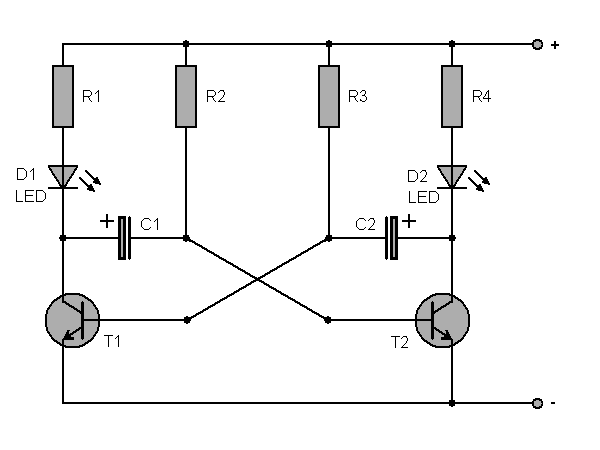
\includegraphics[width=0.70\paperwidth]{./images/multivibrator.png}}}
    \begin{textblock*}{2\paperwidth}(0.65\paperwidth, -0.03\paperheight)
        \vspace*{3.0cm}
        Orientierung (!):
        \begin{itemize}
            \setlength\itemsep{5pt}
            \item LEDs
            \item Transistoren
            \item Kondensatoren (!)
        \end{itemize}
    \end{textblock*}
    \framenumber
\end{frame}


% Elektrische Widerstände: Farbcode
\begin{frame}
    \frametitle{Elektrische Widerstände: Farbcode}
    \AddToShipoutPictureBG*{\put(0.22\paperwidth, 0.06\paperheight){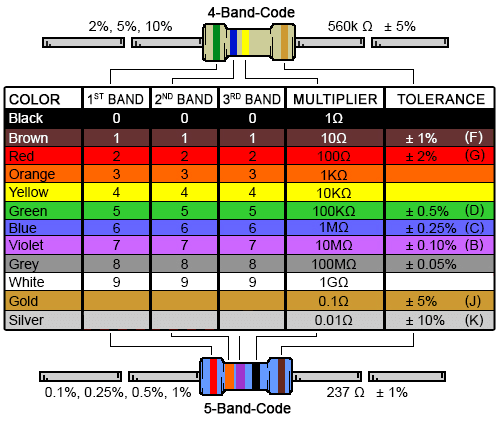
\includegraphics[height=0.80\paperheight]{./images/resistor_color_chart.png}}}
    \begin{textblock*}{1.0\paperwidth}(0.00\paperwidth,0.89\paperheight)
        \begin{center}
            {\fontsize{5}{10}\selectfont[{\fontsize{6}{10}\selectfont D}{\fontsize{4}{10}\selectfont IGIKEY}. URL: https://www.digikey.at/de/resources/conversion-calculators/conversion-calculator-resistor-color-code-4-band. Zugriff. 3. August 2020.]}
        \end{center}
    \end{textblock*}
    \framenumber
\end{frame}


% chapter: Boolsche Algebra
%\begin{frame}[label=boolschealgebra]
%    \chapterslide{\hyperlink{inhalt}{Boolsche Algebra}}
%    \addtocounter{framenumber}{-1}
%\end{frame}


% chapter: Einführung in die FPGA-Programmierung
%\begin{frame}[label=fpga]
%    \chapterslide{\hyperlink{inhalt}{Einführung in die FPGA-Programmierung}}
%    \addtocounter{framenumber}{-1}
%\end{frame}


% VHDL-basierter Entwicklungsprozess
%\begin{frame}
%    \frametitle{VHDL Entwicklungsprozess}
%    % text bullets
%    \begin{textblock*}{2\paperwidth}(0.0\paperwidth,0.0\paperheight)
%        \vspace*{2.0cm}
%        \begin{itemize}
%            \setlength\itemsep{16pt}
%            \item digitale Hardware $\rightarrow$ \textit{Modul}
%            \begin{itemize}
%                \item \textcolor{green}{Bibliotheken}
%                \item \textcolor{blue}{\textit{entity}}
%                \item \textcolor{red}{\textit{architecture}}
%            \end{itemize}
%            \item Softwaretest $\rightarrow$ \textit{Testbench}
%            %\item \textit{nebenläufig} statt sequenziell
%            \item Prozess: \textit{Simulation} $\leftrightarrow$ \textit{Synthese}
%        \end{itemize}
%    \end{textblock*}
%    % image
%    \begin{textblock*}{1.0\paperwidth}(0.975\paperwidth,0.30\paperheight)
%        \rotatebox[origin=c]{90}{{\fontsize{5}{10}\selectfont[{\fontsize{6}{10}\selectfont K}. {\fontsize{6}{10}\selectfont U}{\fontsize{4}{10}\selectfont RBANSKI} et al. \textit{Digitaltechnik}. Berlin. 2015.]}}
%    \end{textblock*}
%    \AddToShipoutPictureBG*{\put(0.58\paperwidth,0.00\paperheight){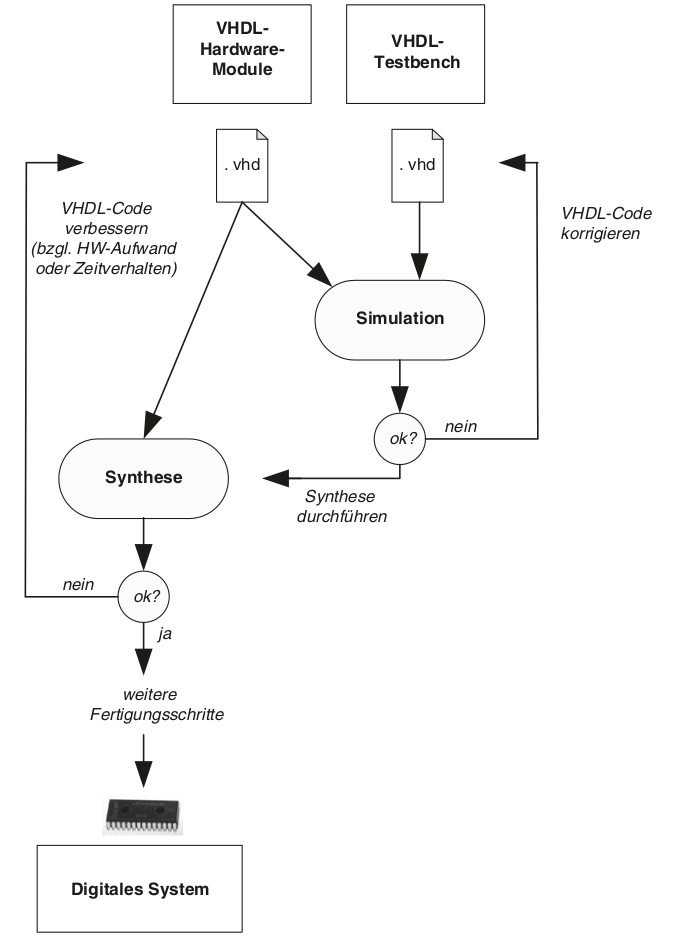
\includegraphics[height=1.0\paperheight]{./images/urbanski__vhdl_basierter_entwurfsprozess.png}}}
%    \framenumber
%\end{frame}


% VHDL-Modul: and-Gate
%\begin{frame}
%    \frametitle{VHDL-Modul: and-Gate}
%    % image source
%    \begin{textblock*}{1.0\paperwidth}(0.975\paperwidth,0.30\paperheight)
%        \rotatebox[origin=c]{90}{{\fontsize{5}{10}\selectfont[{\fontsize{6}{10}\selectfont K}. {\fontsize{6}{10}\selectfont U}{\fontsize{4}{10}\selectfont RBANSKI} et al. \textit{Digitaltechnik}. Berlin. 2015.]}}
%    \end{textblock*}
%    % library
%    \begin{textblock*}{1.0\paperwidth}(0.69\paperwidth,0.20\paperheight)
%        \textcolor{green}{Bibliotheken}
%    \end{textblock*}
%    \AddToShipoutPictureBG*{\put(0.14\paperwidth,0.71\paperheight){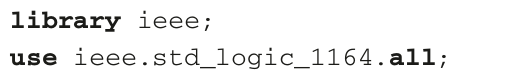
\includegraphics[width=0.53\paperwidth, cfbox=green 1.8pt 0pt]{./images/urbanski__screenshot_and_2_library.png}}}
%    % entity
%    \begin{textblock*}{1.0\paperwidth}(0.69\paperwidth,0.47\paperheight)
%        \textcolor{blue}{\textit{entity}}
%    \end{textblock*}
%    \AddToShipoutPictureBG*{\put(0.14\paperwidth,0.34\paperheight){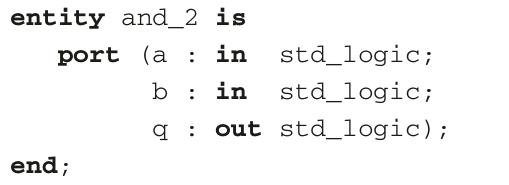
\includegraphics[width=0.53\paperwidth, cfbox=blue 1.8pt 0pt]{./images/urbanski__screenshot_and_2_entity.png}}}
%    % architecture
%    \begin{textblock*}{1.0\paperwidth}(0.69\paperwidth,0.81\paperheight)
%        \textcolor{red}{\textit{architecture}}
%    \end{textblock*}
%    \AddToShipoutPictureBG*{\put(0.14\paperwidth,0.02\paperheight){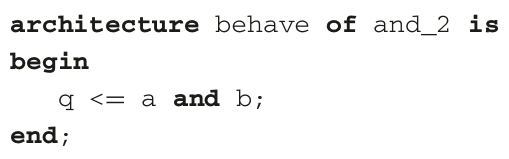
\includegraphics[width=0.53\paperwidth, cfbox=red 1.8pt 0pt]{./images/urbanski__screenshot_and_2_architecture.png}}}
%    \framenumber
%\end{frame}


% Nebenläufigkeit
%\begin{frame}
%    \frametitle{Nebenläufigkeit (\textit{Concurrency})}
%    \begin{textblock*}{2\paperwidth}(0.0\paperwidth,0.0\paperheight)
%        \vspace*{2.0cm}
%        \begin{itemize}
%            \setlength\itemsep{16pt}
%            \item \textcolor{uniblau}{\href{https://stackoverflow.com/questions/13954193/is-process-in-vhdl-reentrant/}{\texttt{stackoverflow}}}
%        \end{itemize}
%    \end{textblock*}
%    \framenumber
%\end{frame}


% Stoppuhr: Arbeitsteilung
%\begin{frame}
%    \frametitle{Die Stoppuhr: Arbeitsteilung}
%    % table
%    \begin{textblock*}{\paperwidth}(0.0\paperwidth,0.62\paperheight)
%        {\fontsize{12}{10}\selectfont
%        \begin{tabular}{C{0.31\paperwidth}C{0.31\paperwidth}C{0.36\paperwidth}}
%        \toprule
%        \toprule
%        SS LED Display  &  BCD Zähler   &   Taktskalierung  \\%[2.0 mm]
%        \midrule
%        Nina        &   Steffi          &   Hany            \\
%        Malte       &   Markus          &   Timo            \\
%        Tim         &                   &                   \\
%        \bottomrule
%        \bottomrule
%        \end{tabular}
%        }
%    \end{textblock*}
%    % bullets
%    \begin{textblock*}{1\paperwidth}(0.0\paperwidth,0.0\paperheight)
%        \vspace*{2.0cm}
%        \begin{itemize}
%            \setlength\itemsep{16pt}
%            \item je Aufbereitung mind. eines VHDL-Moduls
%            \item Erklärung für die Gruppe
%            \item gemeinsame Realisierung der Stoppuhr
%        \end{itemize}
%    \end{textblock*}
%    \framenumber
%\end{frame}


% chapter: Einführung in die Mikrocontroller-Programmierung
%\begin{frame}[label=mikrocontroller]
%    \chapterslide{\hyperlink{inhalt}{Einführung in die Mikrocontroller-Programmierung}}
%    \addtocounter{framenumber}{-1}
%\end{frame}


% Microcontroller vs. Microprocessor
%\begin{frame}
%    %\frametitle{\hspace*{0.8cm} Microcontroller \hspace*{1.2cm} vs. \hspace*{1.2cm} Microprocessor}
%    \frametitle{What is a Microcontroller (MCU)?}
%    % image source
%    \begin{textblock*}{0.6\paperwidth}(0.40\paperwidth,0.9\paperheight)
%        \begin{center}
%            \textcolor{uniblau}{\href{https://www.electronicsforu.com/technology-trends/learn-electronics/difference-between-microprocessor-and-microcontroller}{{\fontsize{5}{10}\selectfont[{\fontsize{4}{10}\selectfont electronicsforum.com} \textit{Microcontroller vs. Microprocessor}. Accessed: 4th March 2021]}}}
%        \end{center}
%    \end{textblock*}
%    \AddToShipoutPictureBG*{\put(0.40\paperwidth,0.07\paperheight){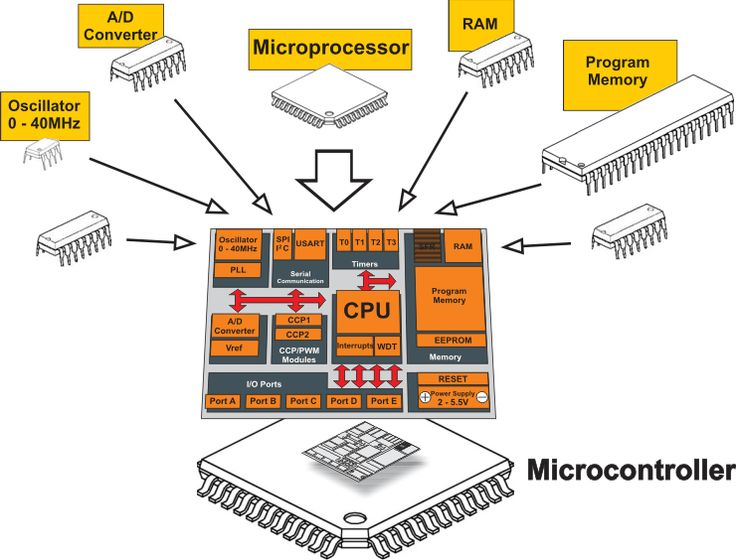
\includegraphics[width=0.55\paperwidth]{./images/what_is_a_microcontroller.jpg}}}
%    % bullet points
%    \begin{textblock*}{2\paperwidth}(0.0\paperwidth,0.0\paperheight)
%        \vspace*{2.5cm}
%        \begin{itemize}
%            \setlength\itemsep{16pt}
%            \item IC
%            \item Hier könnte Ihre Werbung stehen.
%            \item not a Microprocessor (MPU) !
%            \vspace*{-\parskip}
%            \begin{itemize}
%                \setlength\itemsep{1.0mm}
%                \item[$+$]: cost, power consumption, power
%                \item[$-$]: computing power, upgradability
%            \end{itemize}
%        \end{itemize}
%    \end{textblock*}
%    \framenumber
%\end{frame}


% Arduino
%\begin{frame}
%    \frametitle{Arduino}
%    \AddToShipoutPictureBG*{\put(0.23\paperwidth,0.02\paperheight){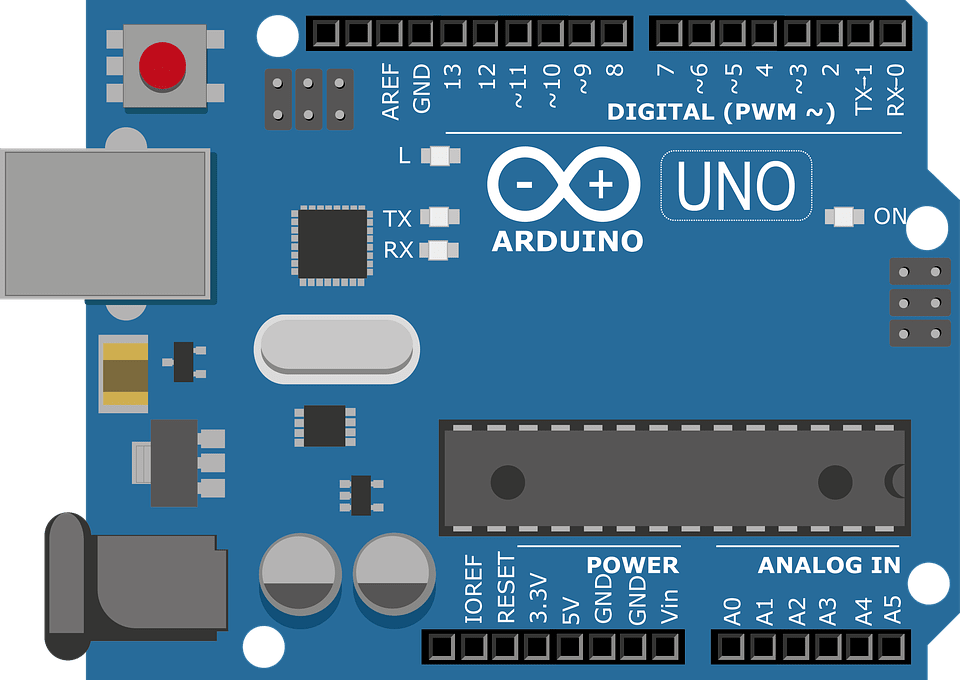
\includegraphics[width=0.75\paperwidth]{./images/arduino_sketch.png}}}
%    \begin{textblock*}{2\paperwidth}(0.0\paperwidth,0.0\paperheight)
%        \vspace*{2.0cm}
%        \begin{itemize}
%            \setlength\itemsep{16pt}
%            \item \textcolor{uniblau}{\href{https://www.arduino.cc/}{Official Webpage}}
%            \item \textcolor{uniblau}{\href{https://www.youtube.com/watch?v=nL34zDTPkcs&t=95s}{\textit{Arduino in 15 minutes}}}
%            \item \textcolor{uniblau}{\href{https://www.conrad.de/de/p/allnet-starterset-starter-kit-uno-r-3-set-atmega328-passend-fuer-arduino-boards-arduino-1359117.html}{EidmDe-Kit}}
%        \end{itemize}
%    \end{textblock*}
%    \framenumber
%\end{frame}


% Arduino: Inspiration & Resources
%\begin{frame}
%    \frametitle{Arduino: Inspiration \& Resources}
%    % inspiration
%    \begin{textblock*}{2\paperwidth}(0.0\paperwidth, -0.03\paperheight)
%        \vspace*{2.0cm}
%        \begin{itemize}
%            \setlength\itemsep{16pt}
%            \item \textcolor{uniblau}{\href{https://www.youtube.com/watch?v=aUbBUd-hBLI}{self balancing robot}}
%            \item \textcolor{uniblau}{\href{https://www.youtube.com/watch?v=T5Aq7cRc-mU}{LED cube}}
%            \item \textcolor{uniblau}{\href{https://www.youtube.com/watch?v=kproPsch7i0}{useless box}}
%            \item \textcolor{uniblau}{\href{https://www.youtube.com/watch?v=xeUl-madZCI}{bluetooth controlled socket}}
%            \item \textcolor{uniblau}{\href{https://www.youtube.com/watch?v=O_Q1WKCtWiA}{garduino}}
%            \item \textcolor{uniblau}{\href{https://create.arduino.cc/projecthub}{\texttt{Arduino project hub}}}
%        \end{itemize}
%    \end{textblock*}
%    % resources
%    \begin{textblock*}{2\paperwidth}(0.5\paperwidth, -0.03\paperheight)
%        \vspace*{2.0cm}
%        \begin{itemize}
%            \setlength\itemsep{16pt}
%            \item \textcolor{uniblau}{\href{https://www.tutorialspoint.com/arduino/index.htm}{\texttt{tutorialspoint}}}
%            \item Beispiel-\textit{Sketches} (IDE)
%            \item \textcolor{uniblau}{\href{https://de.wikipedia.org/wiki/Internet}{DAS INTERNET}}
%        \end{itemize}
%    \end{textblock*}
%    \framenumber
%\end{frame}




% summary 1
%\begin{frame}
%    \summaryslide{Take Home Messages}
%    \begin{textblock*}{2\paperwidth}(0.0\paperwidth,0.0\paperheight)
%        \vspace*{2.0cm}
%        \begin{itemize}
%            \setlength\itemsep{16pt}
%            \item Lötübung $\rightarrow$ Astabile Kippstufe
%            \item Boolsche Algebra $\rightarrow$ logische Gleichungen
%            \item FPGA $\rightarrow$ VHDL-Entwicklungsprozess \& -Stoppuhrprojekt
%            \item Mikrocontroller $\rightarrow$ Arduinoprogrammierung
%        \end{itemize}
%    \end{textblock*}
%    \framenumbersummaryslide
%    \addtocounter{framenumber}{-1}
%\end{frame}
%% effect: feedback QR code
%\begin{frame}
%    \summaryslide{Take Home Messages}
%    \begin{textblock*}{2\paperwidth}(0.0\paperwidth,0.0\paperheight)
%        \vspace*{2.0cm}
%        \hspace*{1.0cm}
%        \textcolor{uniblau}{\href{https://docs.google.com/forms/d/e/1FAIpQLSdAEgryQdZ04KEDBmQFy3ldw4GMcrVsM1QriTker-OboGl9sw/viewform?usp=sf_link}{Feedback $\rightarrow$}}
%    \end{textblock*}
%    \AddToShipoutPictureBG*{\put(0.22\paperwidth,-0.013\paperheight){
\includegraphics[width=0.54\paperwidth]{./images/feedback_query_qr_code.png}}}
%    \framenumbersummaryslide
%\end{frame}

\end{document}






